\documentclass[DIV=calc, paper=a4, fontsize=11pt, twocolumn]{scrartcl}	 
%\usepackage[english]{babel} 
\usepackage[protrusion=true,expansion=true]{microtype} 
\usepackage{amsmath,amsfonts,amsthm} 
\usepackage[svgnames]{xcolor} 
\usepackage[hang, small,labelfont=bf,up,textfont=it,up]{caption} 
\usepackage{booktabs} 
\usepackage{fix-cm}	 
\usepackage{sectsty} 
\allsectionsfont{\usefont{OT1}{phv}{b}{n}}
\usepackage{fancyhdr} 
\pagestyle{fancy} 
\usepackage{graphicx}
\usepackage{grffile}
\usepackage{lastpage}
\lhead{}
\chead{}
\rhead{}
\lfoot{}
\cfoot{}
\rfoot{\footnotesize Page \thepage\ of \pageref{LastPage}} 
\renewcommand{\headrulewidth}{0.0pt} 
\renewcommand{\footrulewidth}{0.4pt} 
\usepackage{lettrine}
\newcommand{\initial}[1]{ 
\lettrine[lines=3,lhang=0.3,nindent=0em]{
\color{DarkGoldenrod}
{\textsf{#1}}}{}}
\newcommand*{\affaddr}[1]{#1}
\newcommand*{\affmark}[1][*]{\textsuperscript{#1}}
\newcommand*{\email}[1]{\texttt{#1}}
%------------------------------
%	TITLE SECTION
%------------------------------
\usepackage{titling} 

\newcommand{\HorRule}{\color{DarkGoldenrod} \rule{\linewidth}{1pt}}
\pretitle{\vspace{-30pt} \begin{flushleft} \HorRule \fontsize{30}{30} \usefont{OT1}{phv}{b}{n} \color{Black} \selectfont} 
\title{Growing Degree Days in Canada}

\posttitle{\par\end{flushleft}\vskip 0.5em}

\preauthor{\begin{flushleft}\large \lineskip 0.5em \usefont{OT1}{phv}{b}{sl} \color{DarkGreen}} 
	
\author{Sara Ayubian\affmark[1]    ,Ghasem Alaee Khangha \affmark[2],    Faramarz Dorani\affmark[3],
Stanley Uche Godfrey\affmark[4],Oluwatosin Adelegan\affmark[5]
Shuyue Qi\affmark[6],Lianbo Li\affmark[7]}
\postauthor{\color{Black} \\
\centering{Memorial University of Newfoundland}\\\centering{\color{Blue}Instructor: Dr.James Munroe} 
\titlepic{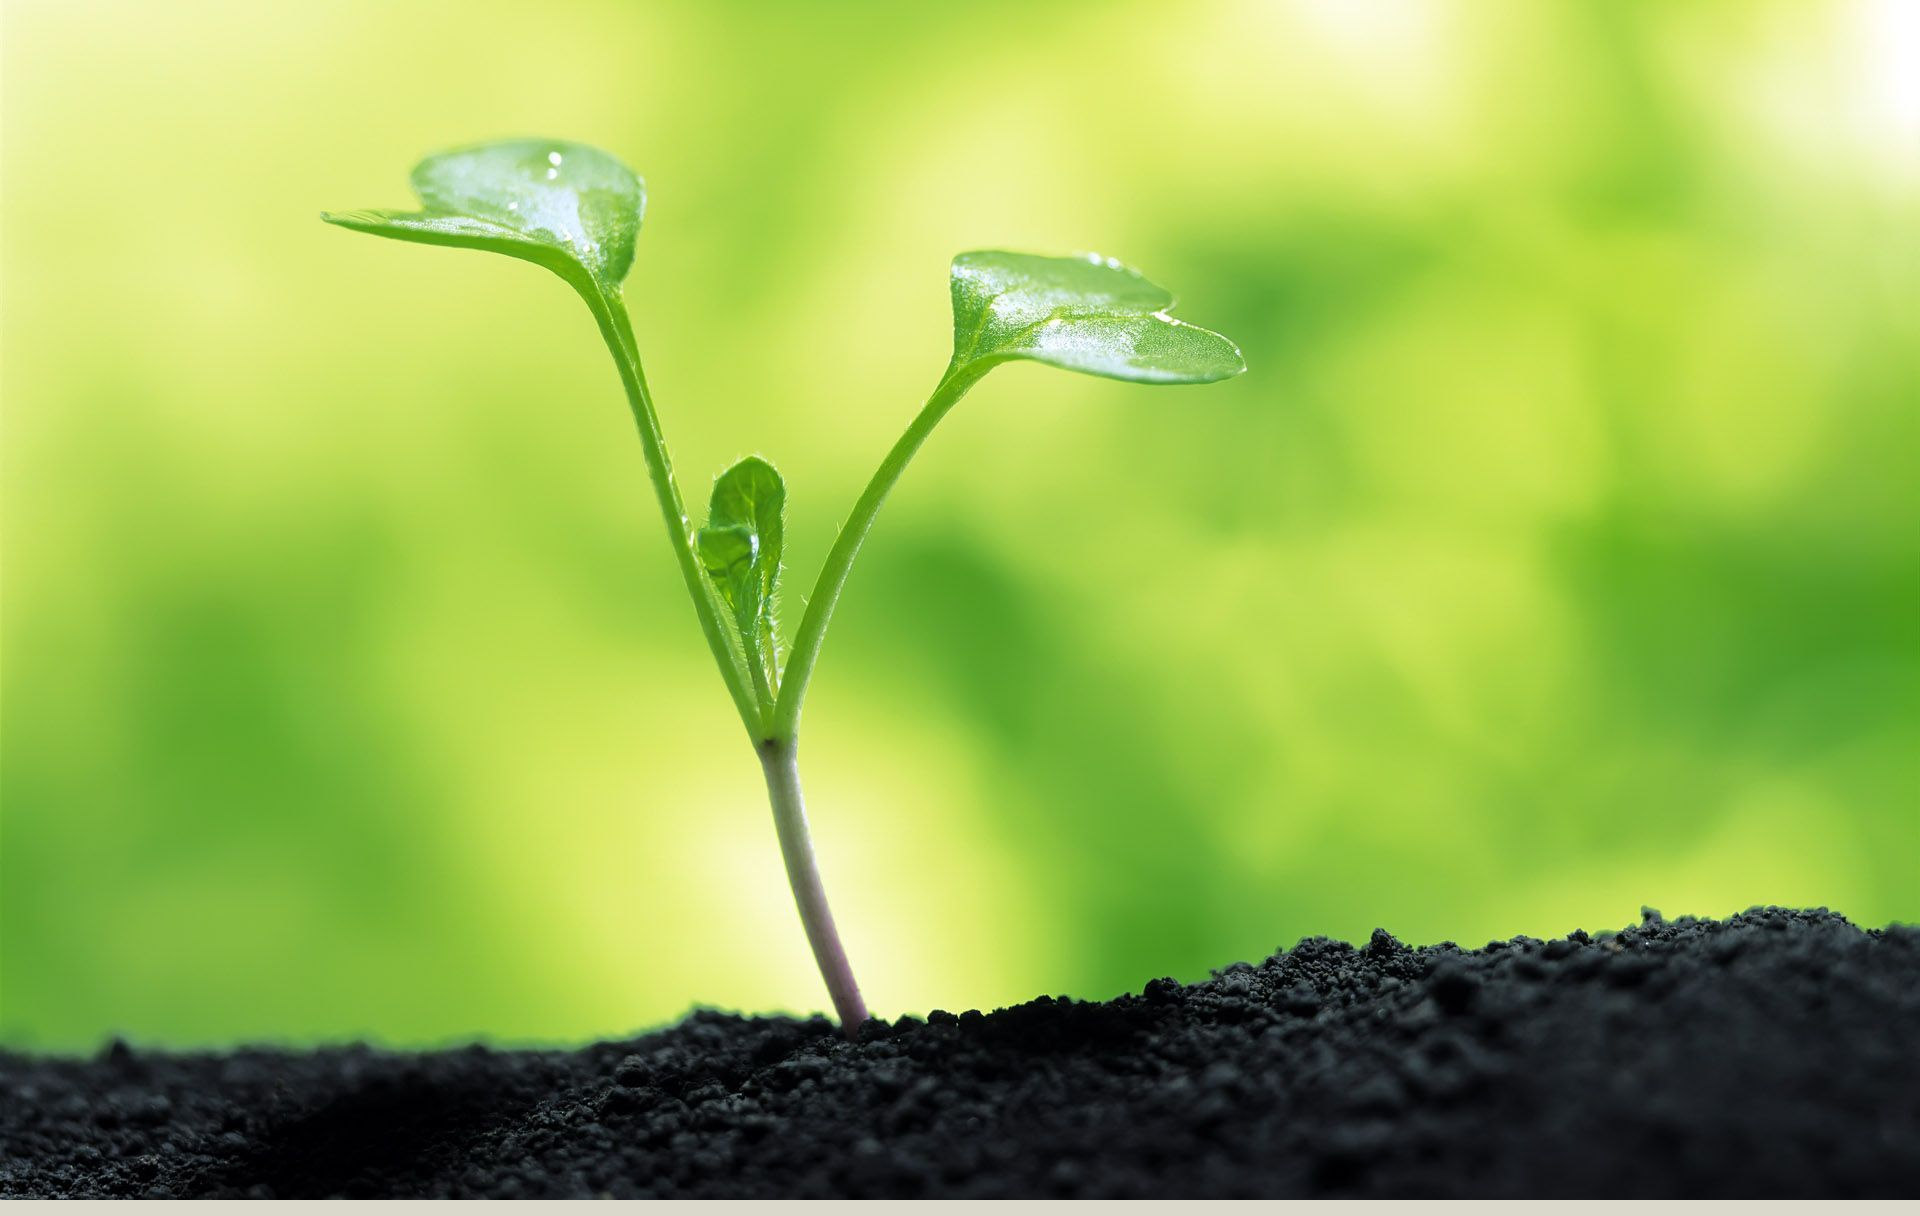
\includegraphics[width=170mm,height=50mm]{GDD.png}}
\\
\centering{Computer Based Research Tools and Application}
\\
\centering{Course Project Report}
\par\end{flushleft}\HorRule}
\date{Spring 2016} 
%-------------------------------------------------------------
\begin{document}
\maketitle 
\thispagestyle{fancy} 
%----------------------------
%	ABSTRACT
%----------------------------
\section{Abstract}

\initial{T}he Growing Degree Day, or GDD, is a heat unit that can be used to predict the timing of biological processes. The present study demonstrates the process of downloading data related to the maximum and minimum temperatures to calculate GDD for three cities (St.John's, Calgary and Toronto) in one years. These steps can be found in http://github.come/sa7818/GDD in a public repository.
	
	
	
%---------------------------
%	ARTICLE CONTENTS
%---------------------------
\section{Introduction}
\subsection{Growing Degree Day}

Heat Unit, can be described by GDD (Growing Degree Days) and it used to express the timing of biological processes. The number of GDD is calculated by subtracting the $T_{base}$ from the average daily temperature for specific plant and animal as follow:
\begin{equation}
GDD =\frac {T_{max}+T_{min}}{2}-T_{base}
\end{equation}

Where $T_{max}$ and $T_{min}$ are daily maximum and minimum air temperature respectively, and $T_{base}$ is the base temperature.\\
To begin with,user needs to download daily historical temperature data for three cities in Canada(St.John's, Calgary and Toronto) from http://climate.weather.gc.ca in one year and extracts those .csv files and save them in related columns, and then these processes can be done by using Python.
The next step for illustrating and analyzing data is to plot GDD for those three cities based on one year which shows the annual cycle of min/max daily tempratures.

The measure of GDD becomes more important as it shows the heat energy available for development and also it demonstrates the biological events that typically occur after a required number of GDDs. The use of GDD is indisputable for agriculture, as farmers can use this measure to determine the maturity of certain species and when their crops should be ready to harvest.

The present study contains command line in order to takes arguments and calculate the GDD for three cities. therefore, we need some functions to implement the actual calculation in order to create plots for accumulated GDD vs time for selected cities.

Last but not least, using version control(git) and collaboration tools (Github) in this project helps to have a better presentation on what we have done so far.


%-----------------------------------------------
\section{Experiment Procedures}
The goal of this study is mainly based on team work to split tasks and learn how to use Github repository to present a scientific research and follow specific rules for the calculation of GDD which those steps are as follow:

\begin{itemize}
\item Automation for downloading tempreture data.
\item Extracting required columns from .csv files.
\item Calculating GDD (via command line program).
\item Storing calculations in .csv files.
\item Creating plot showing an annual cycle of min/max daily temperatures.
\item Producing reports based on the generated plots.
\item Preparing web Presentation.
\end{itemize}
%------------------------------------------------
\section{Results}
The present study worked on three cities in Canada in order to calculate growing degree days for each city and plot them using Python programming. Data have been collected from government page which are available for any years,months,days and hours. 
A summary of the data that was collected during the past year for Calgary, St.John's, and Toronto can be seen in as follow:

\begin{figure}[h!]
	\centering
	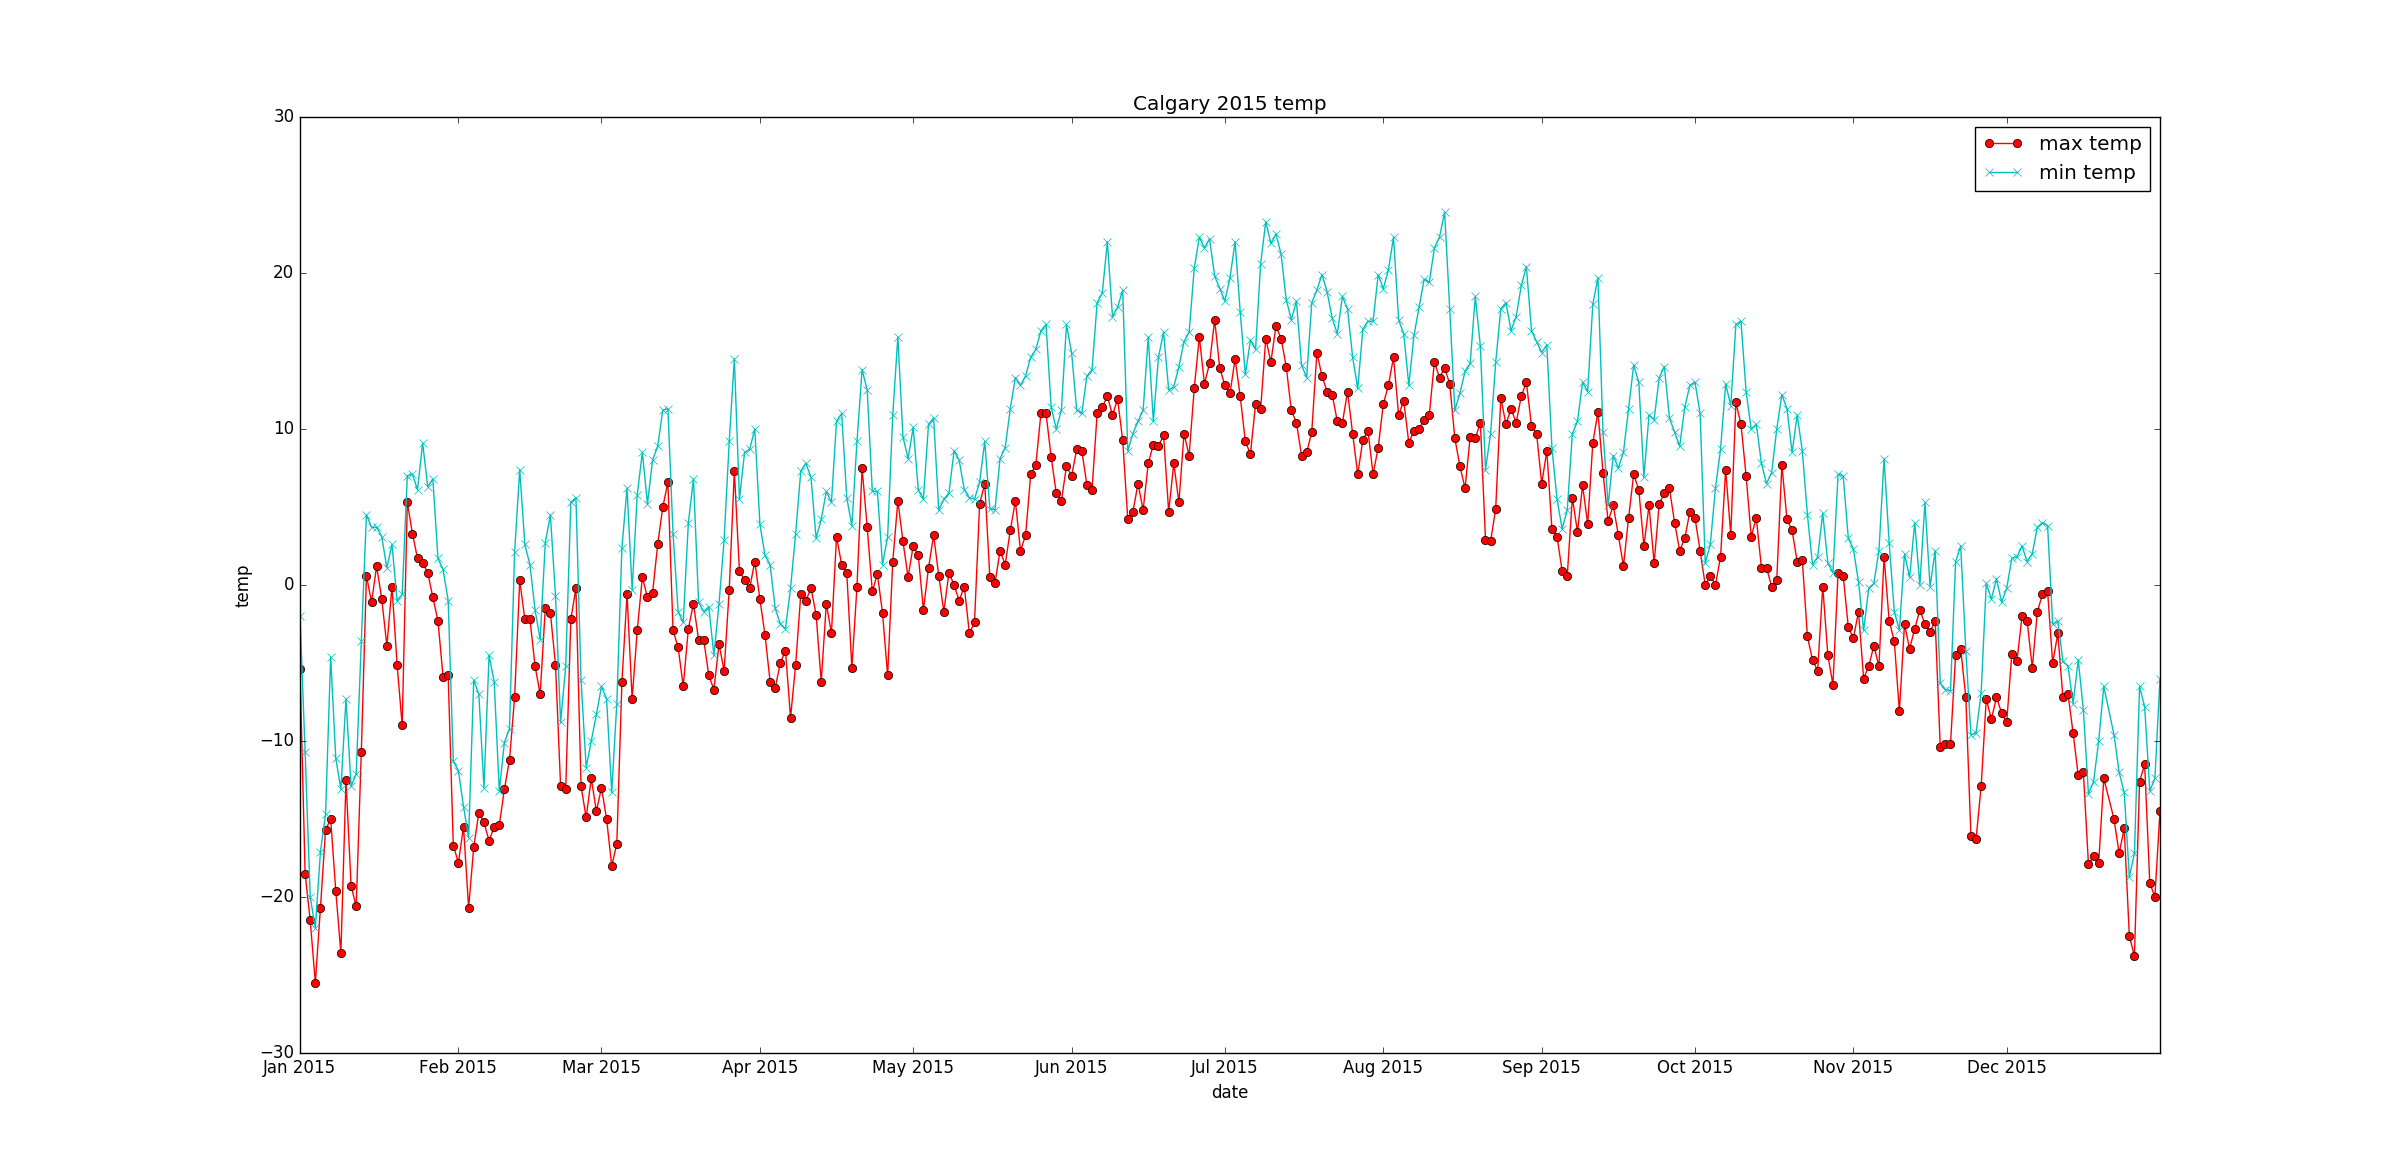
\includegraphics[width=50mm]{../output/plot_images/Calgary_2015.png}
	\caption{Calgary2015}
	\label{fig:method}
\end{figure}
\begin{figure}[h!]
	\centering
	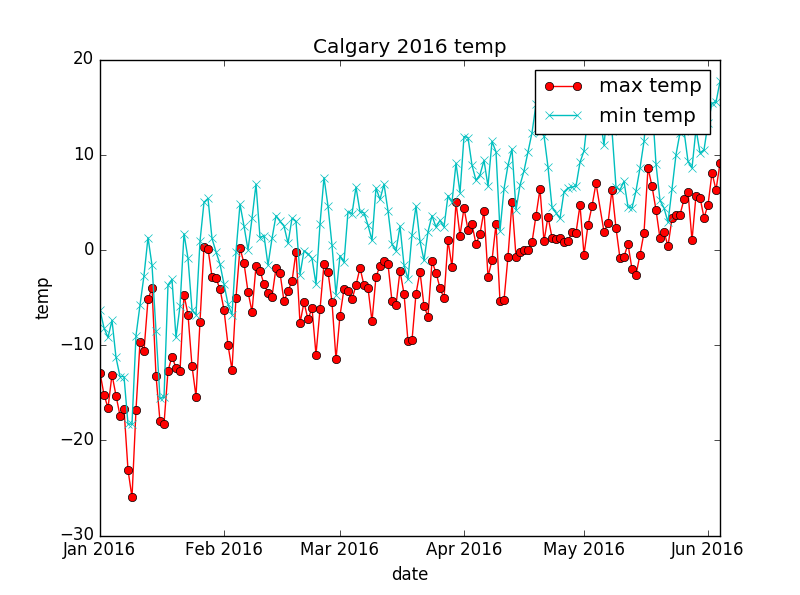
\includegraphics[width=50mm]{../output/plot_images/Calgary_2016.png}
	\caption{Calgary2016}
	\label{fig:method2}
\end{figure}

\begin{figure}[h!]
	\centering
	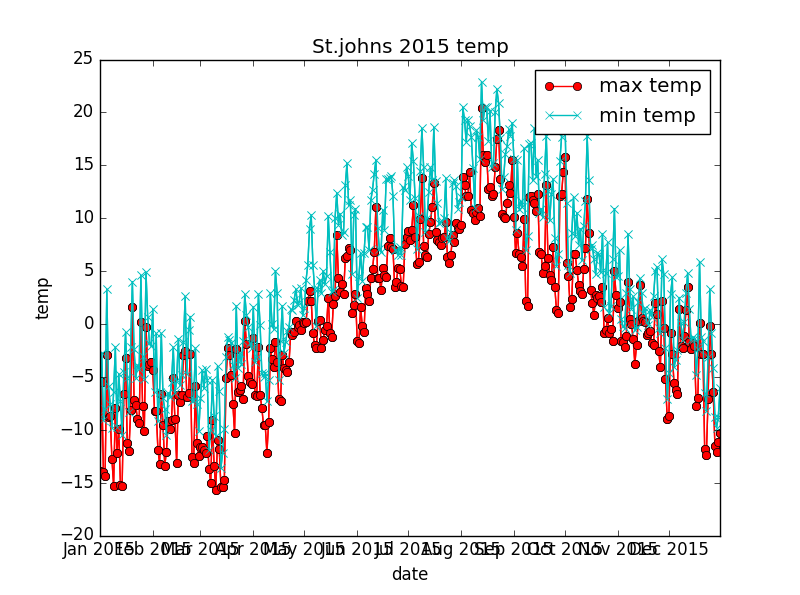
\includegraphics[width=50mm]{../output/plot_images/St.johns_2015.png}
	\caption{St.johns2015}
	\label{fig:method3}
\end{figure}

\begin{figure}[h!]
	\centering
	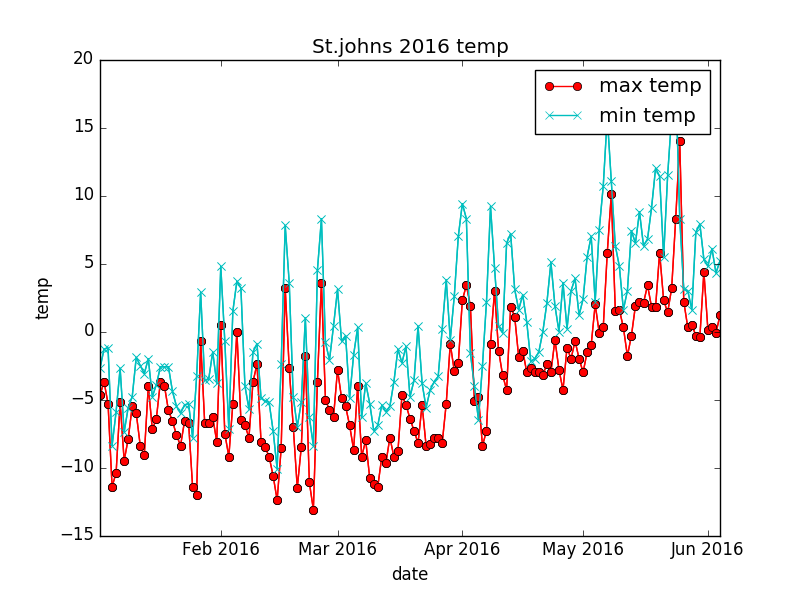
\includegraphics[width=50mm]{../output/plot_images/Stjohns_2016.png}
	\caption{Stjohns2015}
	\label{fig:method4}
\end{figure}
\begin{figure}[h!]
	\centering
	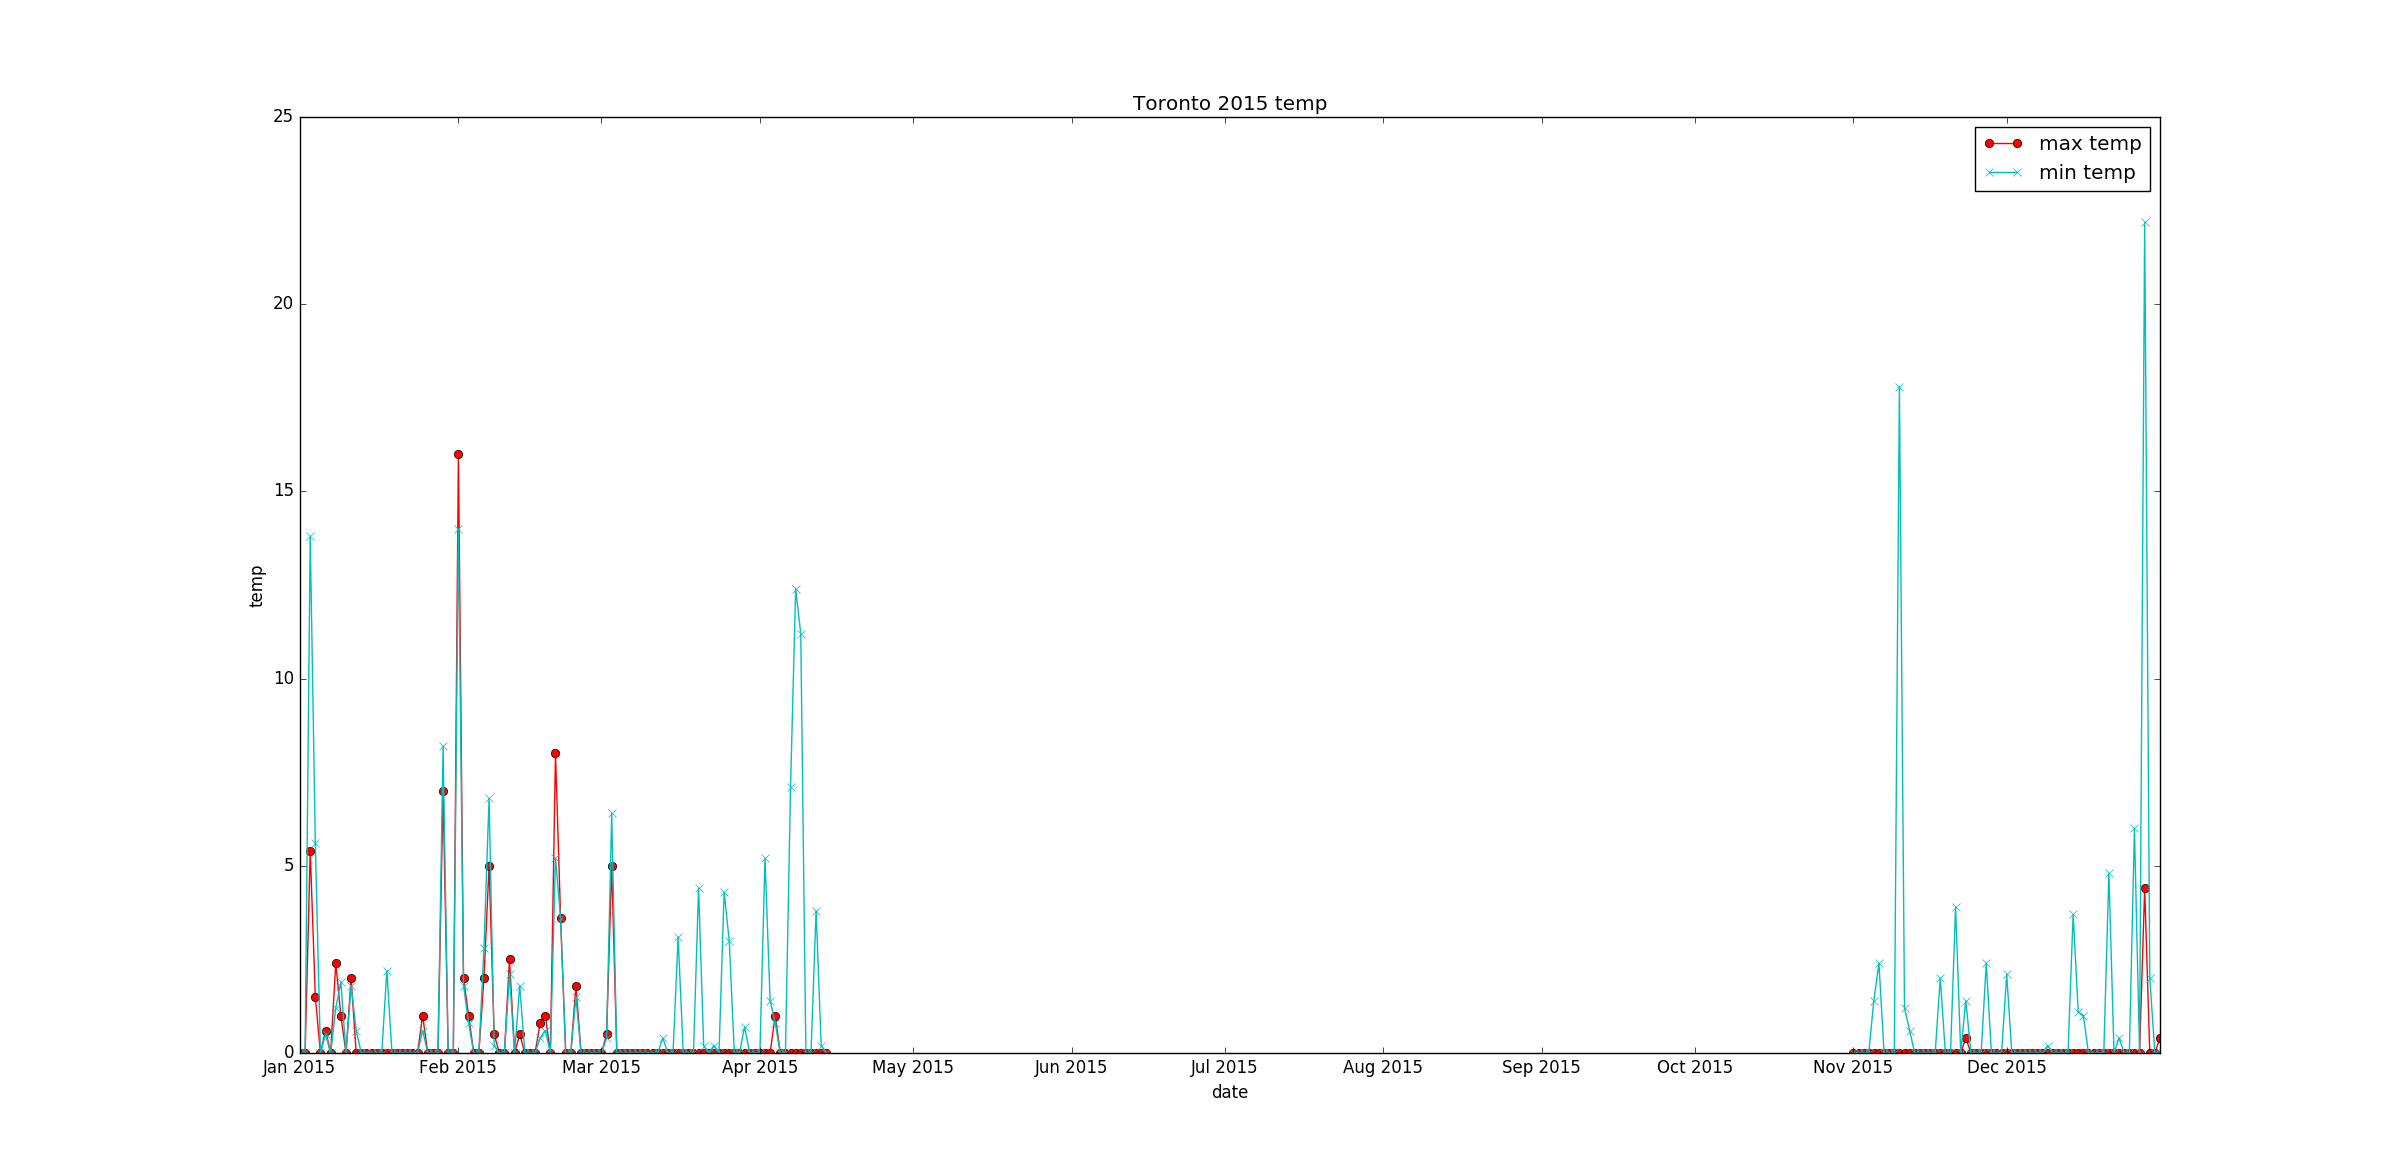
\includegraphics[width=50mm]{../output/plot_images/Toronto_2015.png}
	\caption{Toronto2015}
	\label{fig:method5}
\end{figure}

\begin{figure}[h!]
	\centering
	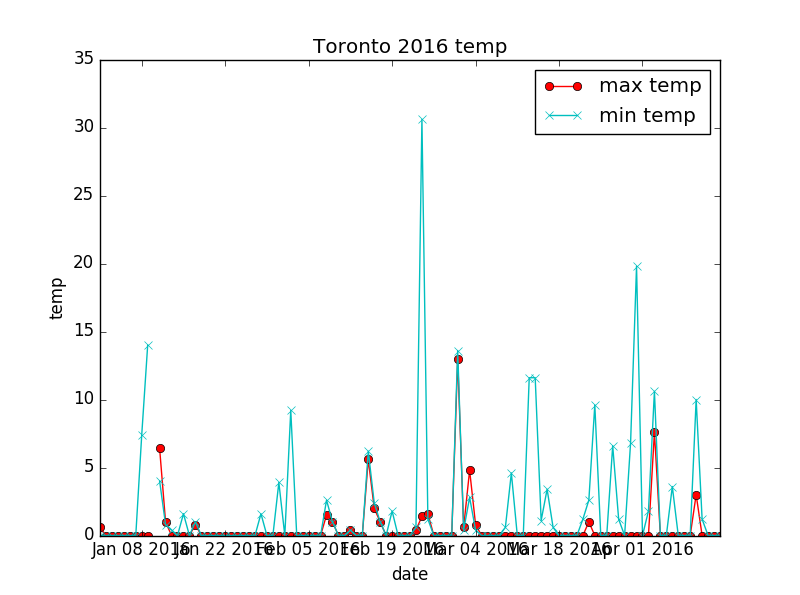
\includegraphics[width=50mm]{../output/plot_images/Toronto_2016.png}
	\caption{Toronto2016}
	\label{fig:method6}
\end{figure}


\section{Conclusion}
The present study has been done by a group of graduate students to show the application of Python programming and many effectives computations in scientifc research. In this experiment, Daily maximum and minimum temperatures were recorded so that GDD could be calculated once all of the data for the one year was collected for three cities, and accumulated GDD were matched with the growth stage of the crop and plots which have been shown in last section demonstrates the result that we have achieved so far.

%-------------------------
%	REFERENCE LIST
%---------------------------

\end{document}